\chapter{Phenomenology of the SDFDM model with real scalars singlets}

\begin{flushright}
This chapter in based in our work published in \textbf{PhysRevD.92.013005 (2015)}\\ 
\url{http://dx.doi.org/10.1103/PhysRevD.92.013005}
\end{flushright}
\begin{center}
\textbf{Abstract}
\end{center}

  \InitialCharacter{W}hen the singlet-doublet fermion dark matter model is extended with
  additional $Z_2$--odd real  singlet scalars, neutrino masses and mixings
  can be generated at one-loop level.  In this work, we discuss the salient 
  features arising from the combination of the two resulting
  simplified dark matter models.  When the $Z_2$-lightest odd particle is a
  scalar singlet, $\operatorname{Br}(\mu\to e \gamma)$ could be
  measurable provided that the singlet-doublet fermion mixing is small
  enough. In this scenario, also the new decay channels of vector-like
  fermions into scalars can generate interesting leptonic plus
  missing transverse energy signals at the LHC. On the other hand, in
  the case of doublet-like fermion dark matter, scalar coannihilations
  lead to an increase in the relic density which allows to lower the bound of
  doublet-like fermion dark matter.








%%%%%%%%%%%%%%%%%%%%%%%%%%%%%%%%%%%%%%
\section{Neutrino masses}

When we extended the SDFDM model with real scalars singlets we were able to get neutrino masses using the realization of the Weinberg operator as it was described in the section~\ref{sec:one-loop masees}.  
In general, is possible to write the neutrino mass matrix~\eqref{eq:neutrino-mass-matrix} as
%
\begin{align}
   M^{\nu}_{ij}=&\sum_{\alpha}\frac{h_{i\alpha}h_{j\alpha}}{16\pi^2}\sum_{n=1}^3 \left( N_{3n} \right)^2m_{\chi_n}
\,f\left( m_{S_\alpha},m_{\chi_n} \right) ,\\\label{eq:Mnuij}
=&\sum_{\alpha} h_{i\alpha} \Lambda_{\alpha} h_{j\alpha}\\\label{eq:CI}
=&\left( \mathbf{h}\mathbf{\Lambda}\mathbf{h}^{\operatorname{T}} \right)_{ij}\,,
\end{align}
with
$f \left( m_1,m_2 \right)= (m_1^2\,\ln  m_1^2 -m_2^2\,\ln m_2^2 )/(m_1^2-m_2^2)$, $\boldsymbol{\Lambda}=\operatorname{Diag}\left(\Lambda_1,\Lambda_2,\Lambda_3\right)$ and
\begin{align}
\label{eq:Lambda}
  \Lambda_\alpha=&\frac{1}{16\pi^2}\sum_{n=1}^3 \left( N_{3n} \right)^2m_{\chi_n}\,f\left( m_{S_\alpha},m_{\chi_n} \right)\,.
\end{align}

As we described in the Appendix~\ref{sec:casas-ibarra}, the flavor structure of the neutrino mass matrix $M^{\nu}_{ij}$, given
by Eq.~\eqref{eq:CI}, allows us to express the Yukawa couplings in
terms of the neutrino oscillation observables (ensuring the proper
compatibility with them) through the Casas-Ibarra parametrization introduced in
\cite{Casas:2001sr,Ibarra:2003up}. 
Thus, by using an arbitrary complex orthogonal rotation matrix
$\boldsymbol{\mathcal{R}}$, the Yukawa couplings $h_{i\alpha}$ are
given by
\begin{align}
  \label{eq:ht}
  \mathbf{h}^{T}=\mathbf{D}_{\sqrt{{\Lambda}^{-1}}}\,\boldsymbol{\mathcal{R}}\,\mathbf{D}_{\sqrt{m_{\nu}}}\,\mathbf{U}^{\dagger} \,,
\end{align}
where $\mathbf{D}_{\sqrt{m_\nu}}=\operatorname{Diag}
\left(\sqrt{m_{\nu 1}} , \sqrt{m_{\nu2}},\sqrt{m_{\nu3}}\right)$,
$\mathbf{D}_{\sqrt{\Lambda^{-1}}}=\operatorname{Diag}
\left(\sqrt{\Lambda_1^{-1}} , \sqrt{\Lambda_2^{-1}},\cdots\right)$ and
$\mathbf{U}$ is the PMNS~\cite{Maki:1962mu} neutrino mixing matrix.

Henceforth, we will consider the case of three scalar singlets, $\alpha=1,2,3$,
where the Yukawa couplings take the form
\begin{align}
\label{eq:Y_CIww}
 h_{i\alpha}=&\frac{\sqrt{m_{\nu 1}}{\mathcal{R}}_{\alpha 1}U_{i1}^*+\sqrt{m_{\nu 2}}{\mathcal{R}}_{\alpha 2} U^{*}_{i2}+ \sqrt{m_{\nu 3}}{\mathcal{R}}_{\alpha 3} U^{*}_{i3}}{\sqrt{\Lambda_\alpha}}\,.
\end{align}
In the above equation, the $3\times3$ matrix
$\boldsymbol{\mathcal{R}}$ can be cast in terms of three rotation
angles $\theta_{23},\theta_{13},\theta_{12}$, which are assumed to be real. 
It is worth mentioning that for the case two scalar singlets
$\alpha=1,2$ a viable scenario is also possible with the remarks that
one massless neutrino is obtained. 
To fully exploit the generality of $h_{i\alpha}$ couplings obtained
from~\eqref{eq:Y_CIww}, we stick to the case with three scalar singlets.

In summary, the set of input parameters of the model are the scalar masses
$m_{S_\alpha}$, $M_N$, $M_D$, $\lambda$,
$\tan\beta$, the lightest neutrino mass $m_{\nu1}$, the three rotation 
angles present in $\boldsymbol{\mathcal{R}}$  
and $\lambda^{SH}_{\alpha\beta}$\footnote{The couplings $\lambda^{S}_{\alpha\beta\gamma\delta}$ are irrelevant for phenomenological purposes.}. Without not loss of generality we assume for the latter to be small $\lambda^{SH}_{\alpha\beta}\lesssim0.01$, except for the case of scalar dark matter where $\lambda^{SH}_{11}$ is set to give 
the proper relic density.

In order to have an approximate expression for $\Lambda_\alpha$ in terms of this set of input parameters, it is possible to use the identity~(\ref{eq:divcan}) to obtain
\begin{align*}
\Lambda_\alpha=&\frac{1}{16\pi^2}\left\{N_{31}^2\,m^\chi_1\left[ f(m_{S_\alpha},m^\chi_1)-f(m_{S_\alpha},m^\chi_3)\right]
                                +N_{32}^2\,m^\chi_2\left[f(m_{S_\alpha},m^\chi_2)-f(m_{S_\alpha},m^\chi_3)\right]\right\}\,.
\end{align*}
The expression for the matrix elements $N_{31}^2$ at $\mathcal{O}\left( m_{\lambda}^2 \right)$ are given in the Appendix~\ref{sec:analyt-form-mass}. Since $N_{31}^2$ and $f(m_{S_\alpha},m^\chi_2)-f(m_{S_\alpha},m^\chi_3)$ are already $\mathcal{O}\left( m_{\lambda}^2 \right)$, we can use the leading order values for the other masses and mixings parameters to obtain
\begin{align*}
  \Lambda_\alpha\approx&\frac{1}{16\pi^2}\left\{N_{31}^2 M_N\left[ f(m_{S_\alpha},M_N)-f(m_{S_\alpha},M_D)\right]
                                +\frac{1}{2}M_D\left[f(m_{S_\alpha},m^\chi_2)-f(m_{S_\alpha},m^\chi_3)\right]\right\}
+\mathcal{O}\left( m_\lambda^4 \right)\,.
\end{align*}
With the last two approximate formula for masses in \eqref{eq:ml2},  and the $N_{31}^2$  mixing in~\eqref{eq:mixl2}, we have
\begin{align}
\label{eq:lambdaappr}
16\pi^2\frac{\Lambda_\alpha}{m_{\lambda}^{2}}\approx & \left(\frac{M_{D} \cos\beta + M_{N} \sin\beta}{M_{D}^{2} - M_{N}^{2}}\right)^{2}
                                  M_{N}\left[f(m_{S_\alpha},M_N)-f(m_{S_\alpha},M_D)\right]\nonumber\\
&+\frac{ M_{D}^{2}\left[M_{D} \sin\left(2 \beta \right ) + M_{N}\right] 
        }{\left(M_{D}^{2} - M_{N}^{2}\right) \left(M_{D}^{2} - m_{S_\alpha}^{2}\right)^{2}} \left\{M_{D}^{2} - m_{S_\alpha}^{2} \left[\log{\left (\frac{M_{D}^{2}}{m_{S_\alpha}^{2}} \right )} + 1\right]\right\}+\mathcal{O}\left( m_\lambda^2 \right)\,.
\end{align}
%
To illustrate the dependence in $\tan\beta$ of $\Lambda_{\alpha}$, we consider the following set of input masses (SIM) compatible with singlet scalar dark matter:
\begin{align}
\label{eq:bp}
  m_{S_1}&=\SI{60}{GeV} & m_{S_2}=&\SI{800}{GeV} & m_{S_3}=&\SI{1500}{GeV}\, \nonumber\\
  m_N&=\SI{100}{GeV} & m_D=&\SI{550}{GeV}\,.
\end{align}
The results for $\lambda=\num{5E-3}$ are shown in
Fig.~\ref{fig:Lambdaa}(a). For large values of $\tan\beta$, the
$\Lambda_{\alpha}$ are positive. However, there are specific values of $\tan\beta$ for which each $\Lambda_{\alpha}$ 
goes to zero and turns to negative values, as illustrated by the red lines in the plot. 
The specific point with $\beta=\pi/6$ is depicted by the yellow stars in the figure.

\begin{figure}
\centering
(a) \hfill (b)\\
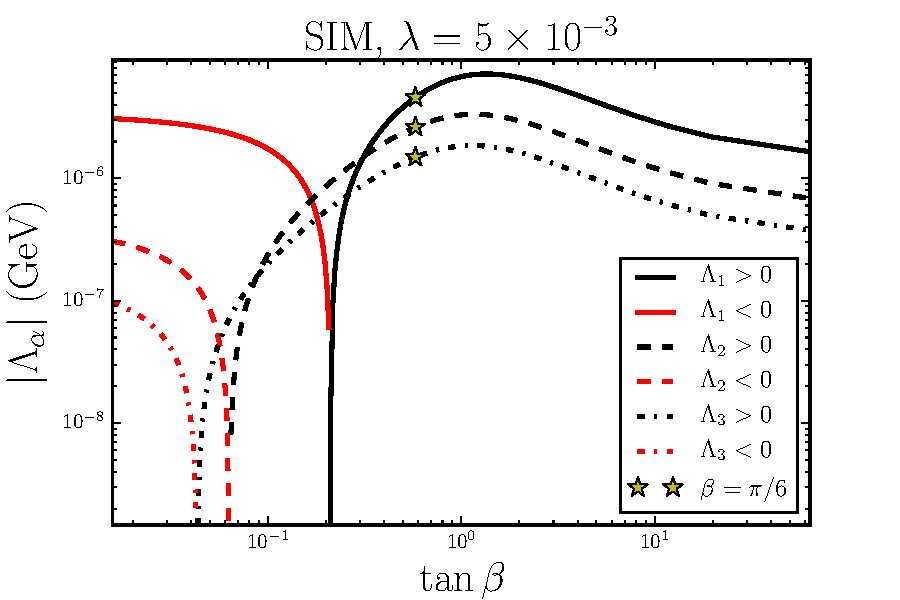
\includegraphics[scale=0.55]{tanbdependence}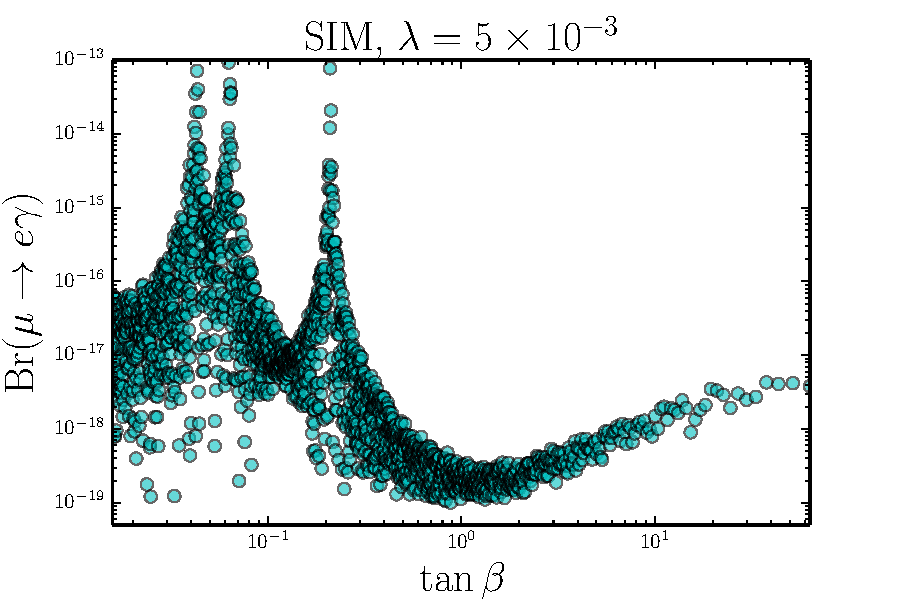
\includegraphics[scale=0.55]{brmuegammatanb}
\caption{$\tan\beta$ dependence of (a) $\Lambda_a$ and (b) $\operatorname{Br}(\mu \rightarrow e \gamma)$, for the set of input masses in Eq.~\eqref{eq:bp} with
$\lambda=\num{5E-3}$.}
\label{fig:Lambdaa}
\end{figure}









%%%%%%%%%%%%%%%%%%%%%%%%%%%%%%%%%%%%%%%%%%%%%%%%%%%%%%%%%%%%%%%%%%%%%%%%%%%%%%%%%%%%%%%%%%%%%%%%%%%%
\section{Lepton flavor violation}
\label{sec:lept-flav-viol}

The size of the lepton flavor violation (LFV) is controlled by the lepton
number violating couplings $h_{i\alpha}$.  
From the approximate expression for $\Lambda_{\alpha}$ found in the Eq.~\eqref{eq:lambdaappr} and the analysis of the previous section, we
will show that these couplings are inversely related to the Yukawa
coupling strength $\lambda$.
Since in SDFDM the observed dark matter abundance is typically
obtained for $\lambda\gtrsim 0.1$~\cite{Cheung:2013dua}, the lepton
flavor observables are not expected to give better constraints than
the obtained from direct detection experiments. Therefore, we will
focus our discussion of LFV in regions of the parameter space
where $S_1$ is the dark matter candidate.

\begin{figure}[h]
\centering
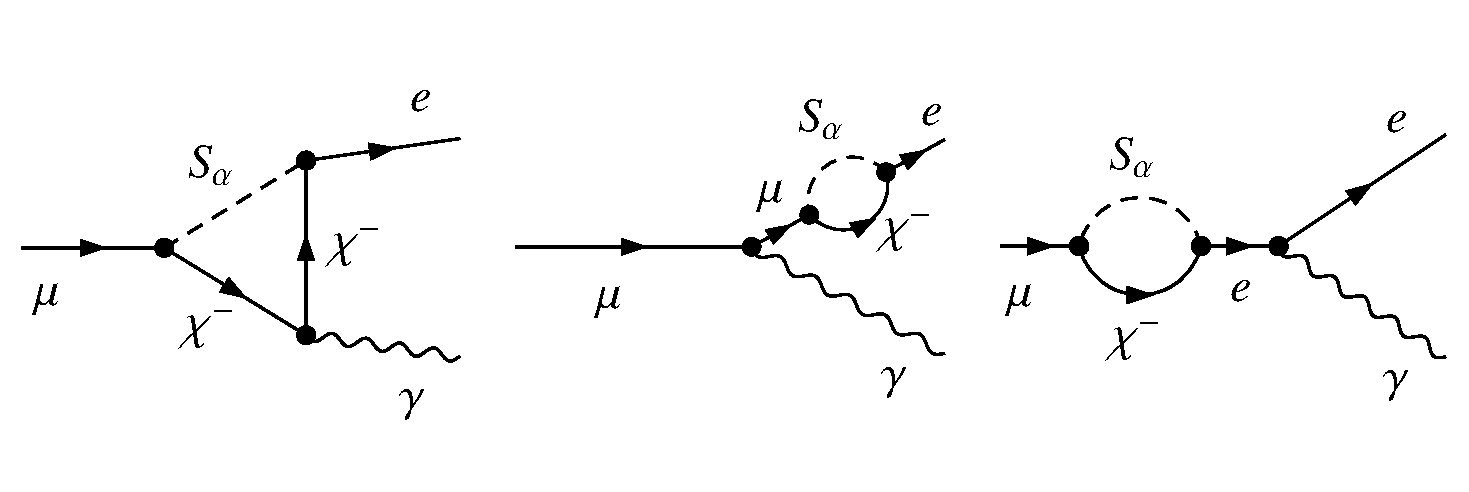
\includegraphics[scale=0.5]{t13a-muegamma1}
\caption{$\mu \to e \gamma$ process generated using \textsc{FeynArts}~\cite{Hahn:2000kx}.}
\label{fig:muegamma}
\end{figure}

It is well known that LFV processes put severe constraints on the LFV
couplings and, in general, on the model's parameter space. 
One of the most restrictive LFV processes is the radiative muon decay
$\mu\to e\gamma$ shown in Fig.~\ref{fig:muegamma}, which in the present model is mediated by same
particles present in the internal lines of the one-loop neutrino mass
diagram shown in Fig.~\ref{fig:T13Aweylme}. 
The corresponding expression for the branching ratio is computed in the Appendix~\ref{sec:Ap-muegamma}. It is given by
%
\begin{align}
\label{eq:muegamma}
\operatorname{Br}(\mu \rightarrow e \gamma)=&\dfrac{3}{4}\dfrac{\alpha_{\text{em}}}{16 \pi G_F^2}\left|\sum_{\alpha}
h_{1\alpha}\frac{F\left(M_D^2/m_{S_{\alpha}}^2  \right) }{m_{S_\alpha}^2}h_{2\alpha}^{*}  \right|^2 ,
\end{align}
where
\begin{align}
F(x)=\dfrac{x^3-6x^2+3x+2+6x\ln x}{6(x-1)^4}\,.
\end{align}
%
With the implementation of the model in the
\texttt{BSM-Toolbox}~\cite{Staub:2011dp} of
\texttt{SARAH}~\cite{Staub:2008uz,Staub:2013tta}, we have crosschecked
the one-loop results for both neutrino masses and $\operatorname{Br}(\mu
\rightarrow e \gamma)$.
Moreover, with the \texttt{SARAH}
\texttt{FlavorKit}~\cite{Porod:2014xia}, we have also checked that the
most restrictive lepton flavor violating process in the scan is just Br($\mu\to e\gamma$).
%
From Eqs.~\eqref{eq:Mnuij} and~\eqref{eq:ht}, we obtain
\begin{align}
  M^{\nu}_{12}=\sum_{\alpha} h_{1\alpha} \Lambda_{\alpha}
  h_{2\alpha}=\left[ \mathbf{U}^{*}\mathbf{M}^{\nu}_{\text{diag}}\mathbf{U}^{\dagger} \right]_{12}\,.%=\sum_{j}m_{\nu j}U_{1j}^{*}U_{2j}^{*}\,.
\end{align}
Comparing this result with the corresponding combination of couplings
in the expression for Br$(\mu\to e\gamma)$ in Eq.~\eqref{eq:muegamma},
we expect that for a set of fixed input masses $\operatorname{Br}(\mu
\rightarrow e \gamma)$ turns out to be inversely proportional to
$\Lambda_\alpha^2$.
This is illustrated in Fig.~\ref{fig:Lambdaa}(b)
for $\lambda=\num{5E-3}$, where the scatter plot of
$\operatorname{Br}(\mu\to e \gamma)$ is shown for the same range of $\tan\beta$ values 
 than in Fig.~\ref{fig:Lambdaa}(a).  In such a case, once
$h_{i\alpha}$ are obtained from the Casas-Ibarra parametrization, the
specific hierarchy of $\Lambda_{\alpha}$ fixes the several contributions
to $\operatorname{Br}(\mu \rightarrow e \gamma)$.  The dispersion of
the points is due to the 3-$\sigma$ variation of neutrino oscillation
data~\cite{Forero:2014bxa} used in the numerical implementation of the Casas-Ibarra
 parametrization, along with the random variation of the parameters of
$\boldsymbol{\mathcal{R}}$. The minimum value of
$\operatorname{Br}(\mu \rightarrow e \gamma)$ around $\tan\beta=1$
corresponds to the maximum value of $\Lambda_{\alpha}$, while the
maximum values happen at the cancellation points of each
$\Lambda_{\alpha}$. In the subsequent analysis, and for a fixed SIM and $\lambda$, we allow 
for cancellations only by two orders of magnitude from the maximum
value of each $\Lambda_{\alpha}$. 

The full scan of the input masses up to $\SI{2}{TeV}$, with
$m_{S_1}>\SI{53}{GeV}$~\cite{Abe:2014gua} as the dark matter candidate,
$M_D>\SI{100}{GeV}$ to satisfy LEP constraints, and
$10^{-2}\le\tan\beta\le 10^2$, give to arise the dark-gray plus
light-gray regions in Fig.~\ref{fig:brmuegamma}. In particular, the
$\lambda$ variation for the SIM with $\beta=\pi/6$, denoted by yellow
stars in Fig.~\ref{fig:Lambdaa}(a), is illustrated
with the white dots in Fig.~\ref{fig:brmuegamma}.   The
corresponding dashed line is obtained for the best-fit values of the
neutrino oscillation data and $\boldsymbol{\mathcal{R}}$ fixed to the
identity. The horizontal dotted line in the plot corresponds to the
current experimental bound for $\operatorname{Br}(\mu\to e
\gamma)<\num{5.7E-13}$ at $90\%\,\si{CL}$~\cite{Adam:2013mnn}.  
The upper part of the 
light-gray region is restricted by our imposition to avoid too strong
cancellation in  $\Lambda_{\alpha}$ . We check that for all the sets of
input masses in the random scan, this cancellation region always
happens when $\tan\beta<1$. In this way, points with $\tan\beta>1$ are
absent from the light-gray region, as labeled in
Fig.~\ref{fig:brmuegamma}. For the same reason, in the dark-gray
region there are not points with $\Lambda_{\alpha}\ll
\Lambda_{\beta}\sim \Lambda_\gamma$ ($\alpha\ne\beta\ne\gamma$). We can check for example that
points with $\Lambda_1\ll \Lambda_2<\Lambda_3$ are absent inside the
dark-gray region of Fig.~\ref{fig:brmuegamma}.


\begin{figure}
  \centering
  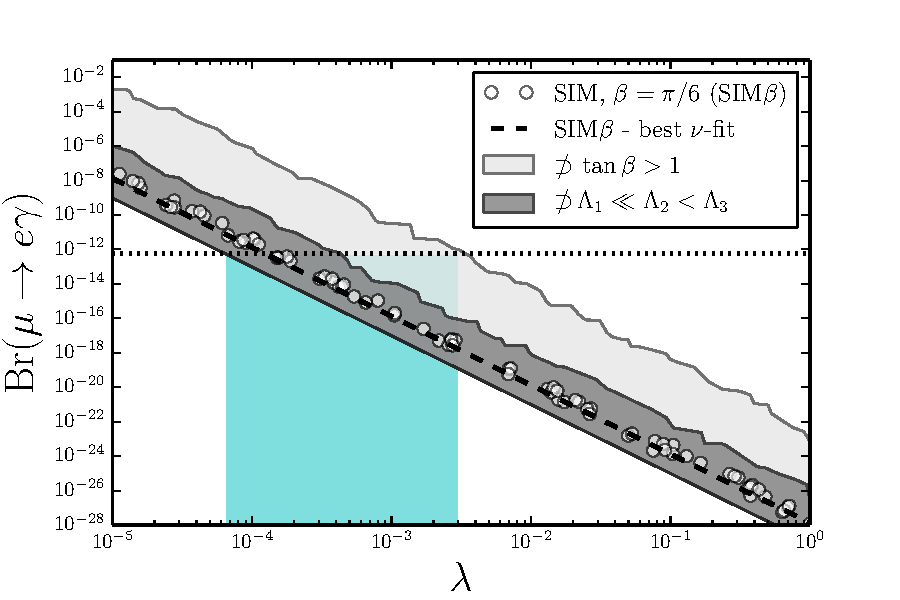
\includegraphics[scale=0.7]{brmuegamma}
  \caption{$\operatorname{Br}(\mu \rightarrow e \gamma)$ in terms of
    the Yukawa coupling strength $\lambda$ for the SIM in
    Eq.~\eqref{eq:bp} with $\beta=\pi/6$, and the general scan
    described in the text.}
  \label{fig:brmuegamma}
\end{figure}



The lower part of the dark-gray region is saturated by the values of
$M_{D}=\SI{2}{TeV}$, and gives rise to the lower bound $\lambda\gtrsim
\num{6E-5}$. 
With our restriction in the cancellation of
$\Lambda_{\alpha}$,  points in the scan with $\lambda\lesssim\num{3E-3}$ 
can be excluded from the Br$(\mu\to e\gamma)$ limit.    









%%%%%%%%%%%%%%%%%%%%%%%%%%%%%%%%%%%%%%%%%%%%%%%%%%%%%%%%%%%%%%%%%%%%%%%%%%%%%%%%%%%%%%%%%%%%%%%%%%%%
\section{Collider phenomenology}
\label{sec:collider-phenomenology}

The LHC phenomenology in the case of the singlet-doublet fermion
dark matter was already analyzed in~\cite{Abe:2014gua}. They concluded that
the recast of the current LHC data is easier to evade, but the
long-run prospects are promising, since the region $M_N,m_\lambda\ll M_D$ could be 
probed up to $M_D\lesssim 600-\SI{700}{GeV}$ for the 14-TeV run of the LHC with 
$\SI{3000}{fb}^{-1}$. 

On the other hand, in the case of the singlet scalar dark matter, the
main production processes associated with the new fermions remain the
same, but there are new signals from the mediation, or presence in the
final decay chains, of the new scalars.
The most promising possibility is the dilepton plus missing
transverse energy signal coming from the production of
charged fermions decaying into leptons and the lightest scalar.
This signal can be important when $\lambda$ is
not too large, $\lambda\lesssim 0.1$, and $M_N\gtrsim M_D$. 
For a fixed set of input parameters, the random phases in the
Casas-Ibarra can be chosen to have all the possibilities in the lepton
flavor space associated with the coupling $h_{i1}$, with
$i=e,\mu,\tau$. 
In view of that, we will focus in the best scenario where
$\operatorname{Br}(\chi^\pm\to l^\pm \, S_1 )\approx 1$ ($l^\pm=e^\pm$ or
$\mu^\pm$). 
The Feynman diagram for the processes is displayed in
Fig.~\ref{fig:chain_signal}.

   
The mass of the  charged  Dirac fermion $\chi^{\pm}$, can be
constrained from dilepton plus missing transverse energy  searches at the  LHC.
In~\cite{Aad:2014vma}, this kind of signals was used by the ATLAS
collaboration to establish bounds on the slepton masses from the
search for $pp \rightarrow \tilde{l}^+\tilde{l}^- \rightarrow l^+l^-
\tilde{\chi}^0\tilde{\chi}^0$, where $\tilde{\chi}^{0}$ are the neutralinos,
and the same exclusion is reported for $l=e$ or $\mu$.
Purely left-handed sleptons produced and decaying this way, have been
excluded up to masses of about $300$ GeV at 95\% CL, from the data
with integrated luminosity of 20.3 fb$^{-1}$ and the $pp$ collision
energy of 8 TeV. 
This corresponds to an excluded cross section of $\SI{1.4}{fb}$ at NLO
calculated with \texttt{PROSPINO}~\cite{Beenakker:1996ed}.

In the present model, the charged fermion field may decay in the
mode $\chi^{\pm} \rightarrow e_i^{\pm}S_1$ which are
proportional to the Yukawa couplings $h_{i1}$. 
Therefore, a similar final state as in the slepton pair production is
obtained through the process $pp \rightarrow \chi^+\chi^- \rightarrow
l^+l^- S_1 S_1$, as can be seen in Fig.~\ref{fig:chain_signal}.


\begin{figure}[h]
\begin{center}
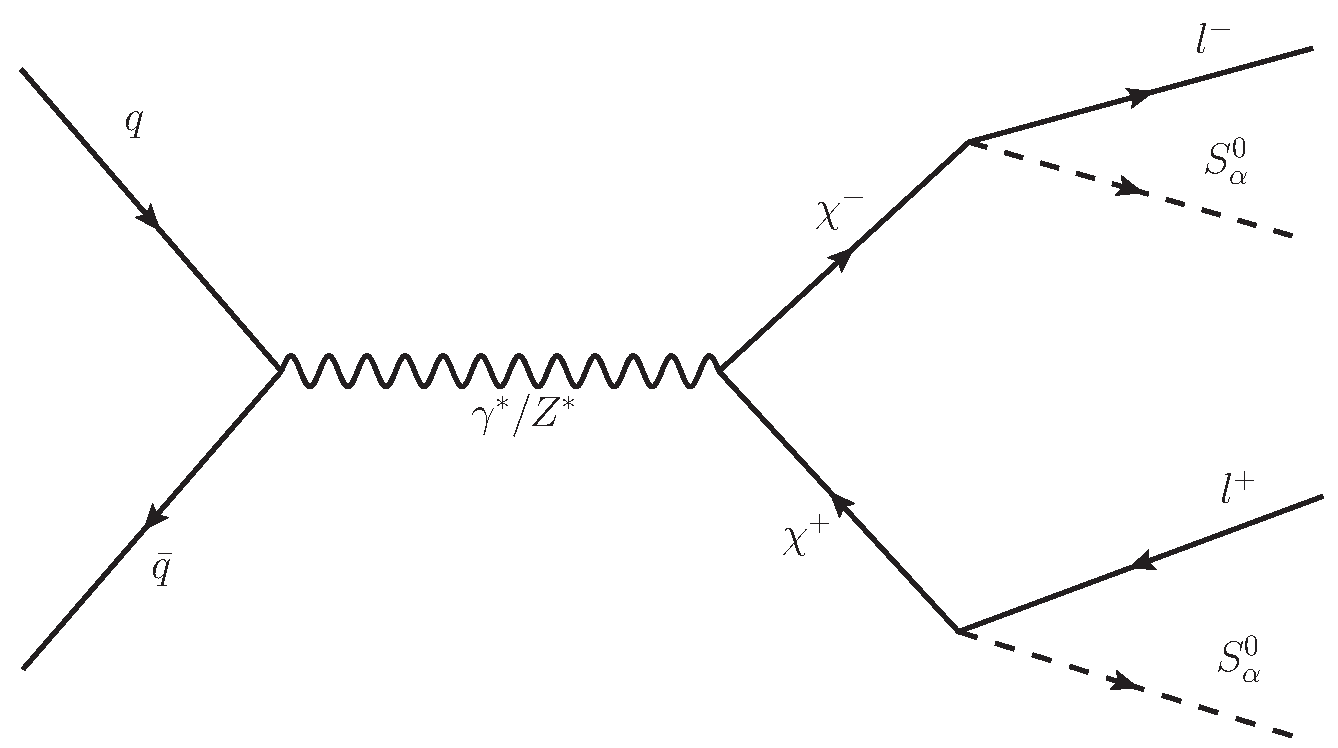
\includegraphics[scale=0.4]{chain1}
\caption{Feynman diagram for $pp \rightarrow \chi^+\chi^- \rightarrow l^+l^- S_{\alpha}S_{\alpha}$ (Drell-Yan process).}
\label{fig:chain_signal}
\end{center}
\end{figure}

In this case, the excluded cross section of this process can be estimated from:

\begin{align}
\label{eq:exccs}
\sigma(pp \rightarrow l^+l^-S_1 S_1)=\sigma(pp \rightarrow \chi^+\chi^-)\times \operatorname{Br}(\chi^{\pm} \rightarrow l^{\pm}S_1)^2 ,
\end{align}
where $\sigma(pp \rightarrow \chi^+\chi^-)$ is the pair production
cross section of charged Dirac fermion, and
$\operatorname{Br}(\chi^{\pm} \rightarrow l^{\pm}S_1)$ is the
branching fraction for $\chi^{\pm} \rightarrow l^{\pm}S_1$
mode.

The pair production of charged Dirac fermions can be
calculated in the pure-higgsino limit of the minimal supersymmetric
standard model. 
The NLO cross section calculated with \texttt{PROSPINO} is displayed
in Fig.~\ref{fig:chargino_production} as a function of the charged
Dirac fermion.

For points in the parameter space where the Casas-Ibarra solution is
chosen such that $\operatorname{Br}(\chi^\pm\to l^\pm\,S_1)\approx 1$,
and assuming the same efficiency as for the dilepton plus missing
transverse energy signal coming from left-sleptons in
Eq.~\eqref{eq:exccs}, the charged Dirac fermions of the present model
can be excluded up to $\SI{510}{GeV}$, as illustrated in
Fig.~\ref{fig:chargino_production}.

\begin{figure}[h]
\begin{center}
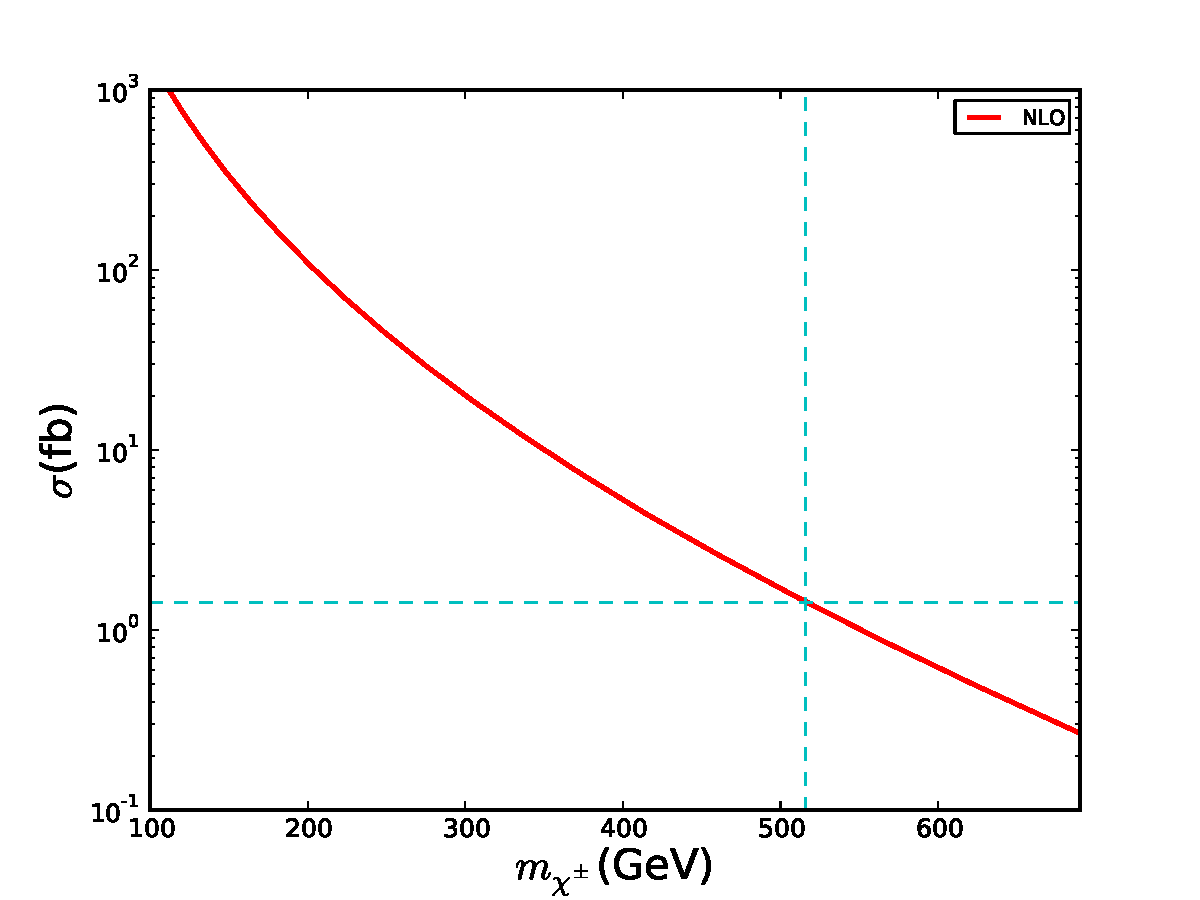
\includegraphics[scale=0.5]{cs2_chacha_prospino}
\caption{NLO cross section for the charged Dirac fermion pair
  production at the LHC with $pp$ collisions at $\sqrt{s}=8$ TeV. 
  The horizontal dashed line for the excluded cross section of
  $\SI{1.4}{fb}$, corresponds to the mass about $\SI{510}{GeV}$
  illustrated by the vertical dashed line.}
\label{fig:chargino_production}
\end{center}
\end{figure}

Note that many points in the scan of Fig.~\ref{fig:brmuegamma} with
$\lambda\lesssim 0.1$ and featuring $m_{S_1}\ll M_D$, could be
excluded by this LHC constraint. 
However, a detailed analysis of the restriction from the Run~I of the
LHC, in the full parameter space of the model, is beyond the scope of this
work.












%%%%%%%%%%%%%%%%%%%%%%%%%%%%%%%%%%%%%%%%%%%%%%%%%%%%%%%%%%%%%%%%%%%%%%%%%%%%%%%%%%%%%%%%%%%%%%%%%%%%
\section{Coannihilation }
\label{sec:singlet-doublet-dark}
In this model, the role of the dark matter particle can be played by
either the lightest of the fermions $\chi_{\text{LOP}}$ or the lightest of the
scalars $S_1$. 
In the latter case, the present model resembles the
singlet scalar DM model
\cite{Silveira:1985rk,McDonald:1993ex,Burgess:2000yq} as long as the
other $Z_2$-odd particles do not contribute to the total annihilation
cross section of $S_1$, namely through to the addition of new
(co)annihilation channels. 
Therefore, by choosing a non-degenerate mass spectrum and small Yukawa
couplings (which is in agreement with neutrino masses) the effects of these particles on dark matter can be neglected. 
Hence, we expect that the dark matter phenomenology to be similar to
that of the SSDM \cite{Cline:2013gha}. 

On the other hand, regarding the case of fermion DM, the present model includes the
singlet doublet fermion DM model
\cite{ArkaniHamed:2005yv,Mahbubani:2005pt,D'Eramo:2007ga,Enberg:2007rp,Cohen:2011ec,Cheung:2013dua}.
In such a scenario, when the dark matter candidate is mainly singlet
(doublet), the relic density is in general rather large (small). 
In particular, a pure doublet has the proper relic density for
$M_{D}\sim\SI{1}{TeV}$~\cite{Mahbubani:2005pt,Cheung:2013dua,Chattopadhyay:2005mv}
with decreasing  values as $M_D$ decreases.  
Nonetheless, in the present model, we have the additional possibility
of coannihilations between the $Z_2$-odd scalars and fermions. 
In this work, we explore at what extent coannihilation with
scalars may allow recovering pure-doublet DM regions with
$M_D\lesssim\SI{1}{TeV}$ and $\lambda\lesssim0.3$ while keeping the
proper relic density.  
Hereafter, we focus in that specific region.


In the simple radiative seesaw model with inert
doublet scalar dark matter, the coannihilations with singlet fermions can enhance
rather than reduce the relic density, as shown in~\cite{Klasen:2013jpa}. That work also presented a review of the several
models~\cite{Servant:2002aq,Kong:2005hn,Burnell:2005hm,Edsjo:2003us,Profumo:2006bx}
where such an enhancement also occurs.
In particular, supersymmetric models where
the neutralino is higgsino-like were considered in~\cite{Profumo:2006bx} and it
was shown that slepton coannihilations not only lead to an increase in
the relic density but also to an enhancement in the predicted
indirect detection signals. 
Below, we show that the singlet scalars can play the role of the
sleptons in our generalization of the higgsino-like dark matter with
radiative neutrino masses.


\begin{figure}
  \centering
  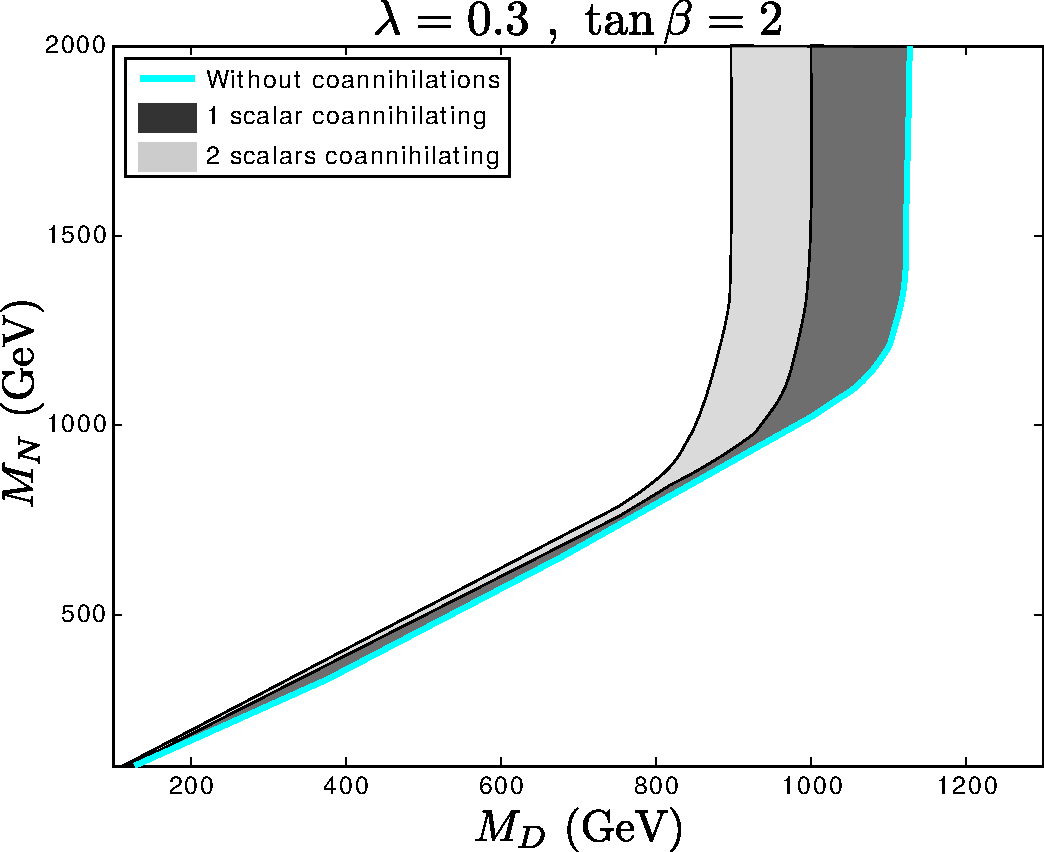
\includegraphics[scale=0.5]{sdfdm}
  \caption{Regions consistent with the observed relic density for $\lambda=0.3$
   and $\tan\beta=2$.    The solid cyan line corresponds to the observed relic density
   without coannihilations which were shown to be compatible with the
   current direct detection bounds from LUX~\cite{Akerib:2013tjd}
   in~\cite{Cheung:2013dua}.
   The effect of the coannihilations with the new scalars is shown for
   a mass degeneracy of 0.1 to 10\% between the scalars and the DM
   candidate. 
   The dark-gray region corresponds to coannihilations with one scalar
   singlet, while the dark plus light-gray regions correspond to
   coannihilations with two scalar singlets.  }
  \label{fig:5b}
\end{figure}


The interactions of the scalars $S_\alpha$ are described by the
$h_{i\alpha}$, $\lambda_{\alpha\beta}^{SH}$ terms in
Eq.~\eqref{eq:lt13a}. 
It turns out that Yukawa interactions are suppressed by neutrino
masses ($h_{i\alpha}\lesssim10^{-4}$) and the same occurs for the interaction
with the Higgs boson if we impose
$\lambda_{\alpha\beta}^{SH}\lesssim10^{-2}$.
In this way, the coannihilating scalars $S_\alpha$ act as parasite
degrees of freedom at freeze-out, leading to an increase of the
singlet-doublet fermion relic density. 

By following the discussion in~\cite{Klasen:2013jpa}, the maximum
enhancement of the relic density is achieved when
$\Delta_{S_\alpha}=(m_{S_{\alpha}}-m_{\text{LOP}}^{\chi})/m_{\text{LOP}}^{\chi}$
becomes negligible. 
Accordingly, one can write
\begin{align}
\frac{  \Omega^{S_{\alpha}}}{\Omega^{0}}\approx\left( \frac{g_0+g_{S_{\alpha}}}{g_0} \right)^2,
\end{align}
where $\Omega^{S_{\alpha}}$ ($\Omega^{0}$) denotes the relic density
with (without) including $S_{\alpha}$ coannihilations,
$g_{S_{\alpha}}$ represents the total number of internal degrees of
freedom related to the scalars participating in the in the
coannihilation process, and $g_{0}$ is the total number of internal
degrees of freedom when $\Delta_{S_\alpha}\gg1$. 
When the DM particle is pure doublet ($M_D\sim1$ TeV and $M_N\gg M_D$),
the fermion masses are $m_1^{\chi}=M_N,\,m_{2,3}^{\chi}\approx
m_{\chi^\pm}=M_D$ and therefore
$g_{0}=g_{\chi_2}+g_{\chi_3}+g_{\chi^\pm}=8$.
Since each real scalar has one degree of freedom, we have
$g_{S_{\alpha}}=1,2,3$ depending on the number of scalars
coannihilating. Thus, it follows that the maximum enhancement is
$\Omega^{S_{\alpha}}/\Omega^{0}=1.27,\, 1.56,\,1.89$, respectively. 
This enhancement results in that, for the present model with
doublet-like DM and $\lambda\lesssim0.3$, the $M_D$ required to explain
the correct relic density lies in the range $[0.9,1.1]$~TeV instead of
taking a single value as in the SDFDM model.  
The values inside this range arise due to no mass-degeneracy
between the fermions and scalars. 
In Fig.~\ref{fig:5b}, we show the effect of coannihilations on the
relic density~\footnote{The relic density is calculated with the
  \texttt{BSM-Toolbox} chain: 
\texttt{SPheno}~3.3.6~\cite{Porod:2011nf}-\texttt{MicrOMEGAs}~4.1.7~\cite{Belanger:2006is,Belanger:2014vza}.}
of $m_{\text{LOP}}^{\chi}$ for a mass degeneracy of 0.1
to 10\% between  scalar singlets and the DM candidate and for
$\lambda=0.3$ and $\tan\beta=2$. 
In particular, in the light-gray region, we plot the coannihilations
with two scalars to facilitate the comparison with the results
in~\cite{Profumo:2006bx} for higgsino-like dark matter coannihilating
with a right-handed stau ($g\approx 2$ in their plots).
As expected, the upper limit in the LOP mass is about $20\%$ smaller
with respect to the case without coannihilation, and we could 
expect similar enhancements for indirect DM searches
as  in ~\cite{Profumo:2006bx} for $g\approx 2$.
Note that, when $M_D,\,M_N<\SI{1}{TeV}$, the impact of the $S_\alpha$ coannihilation is reduced because, in such case, the
dark matter particle is a mixture of singlet and doublet
(well-tempered DM \cite{ArkaniHamed:2006mb}), and the non-negligible
splitting among the fermion particles $\chi$ leads to a non-zero
Boltzmann suppression. 
We have checked that the same results are obtained when
$\lambda\lesssim0.3$.

With regard to DM direct detection in the pure-doublet DM scenario
discussed above, it is not restricted by the current LUX~\cite{Akerib:2013tjd} bounds as
long as $\tan\beta>0$.  
This is due to the existence of zones, known as blind spots, where the
spin-independent cross section vanishes identically and they occur
only for positive values of $\tan\beta$
\cite{Cheung:2013dua}\footnote{Note that $\tan\beta>0$ corresponds to
  $\tan\theta<0$ in notation of  \cite{Cheung:2013dua}.}. 
In consequence, the recovered pure-doublet DM regions are still viable
in light of the present results of direct searches of dark matter.  
%%%%%%%%%%%%%%%%%%%%%%%%%%%%%%%%%%%%%%%%%%%%%%%%%%%%%%%%%%%%%%%%%%%%%%%%






